\documentclass{article}
\usepackage{graphicx}
\renewcommand{\baselinestretch}{2.0}
\begin{document}

\title{Lab 2 Part 1 }
\author{Daniel Ocampo}

\maketitle
\begin{enumerate}
    
\section{Questions in Red}    

\item How many people have used the web site since last month?
I did not get any last month because I messed up the setting that only allowed Allegheny user to access the website.
\item  Where were these users from (country and city)?
Today I was able to find people from San Bruno, California, and Meadville PA.  
\item  Which pages did they read?
The most read pages was the first one and from their the pages ranged. 
\item  What was the highest bounce rate?
The highest bounce rate was 28.57, and think that was because the site was not finished yet when it was published. 
\item  How many visits were there?
there were about 95 visits, by 10 visitors.  
\item  Number of unique visitors?
0, I did not get any unique visitors.  
\item  Number of page views?
I got 95 page views. 

\item  Average visit duration?
The average session for the site was 3:02.  

\item  Percentage of new visits?
52.4 percent were new viewers. 
\item  Percentage of search traffic?
Not sure what this means 
\item  How did this traffic come to the website?
Most of my traffic came from Facebook. 

\end{enumerate}


\newpage
\section{Tutorial}
\subsection{homepage} 

Google analytic is a tools that monitors who, and how long a person has been using your data. In \textbf{Figure 1}, We have a graph that shows you how many people have used your Websites,  the same person can have more than 1 device so we should also note that it can skew the data for new users.
\begin{figure}[t]
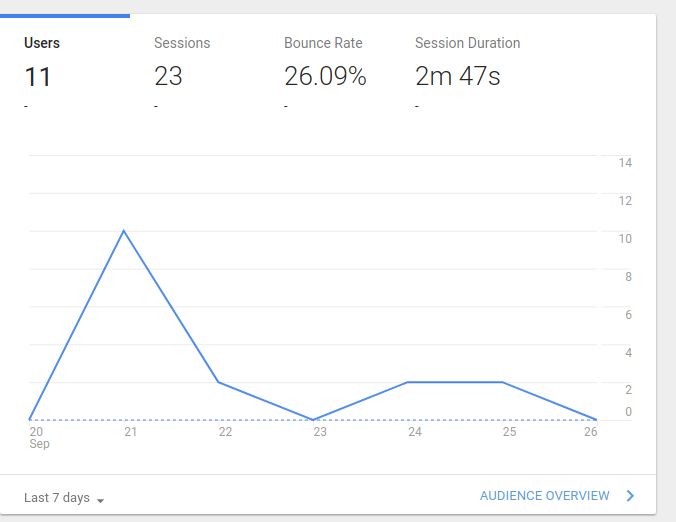
\includegraphics[width=8cm]{users}
\centering
\caption{Number of Users}
\end{figure}
In \textbf{Figure 1}, shows that the website had 11 new users, but keep in mind that some users could have accessed the website through a different device. In the case that we want to find where all of these user are coming from, Google analytics allows the user to find the location of every user. In \textbf{Figure 2}, we see a map of all of people that accessed your website from all of the united states, we do so by going to location overview, which should be underneath User active right now, of the home page. Now we know what part of the country all of users come from. In \textbf{Figure 2 }, we can clearly see that all of our users are from the US. Now if we want to to know if we what part of the US did all of user came from we can just easily click on the United State, Which is shaded blue. This will take us to the parts of the US that accessed the website.
\begin{figure}[t]
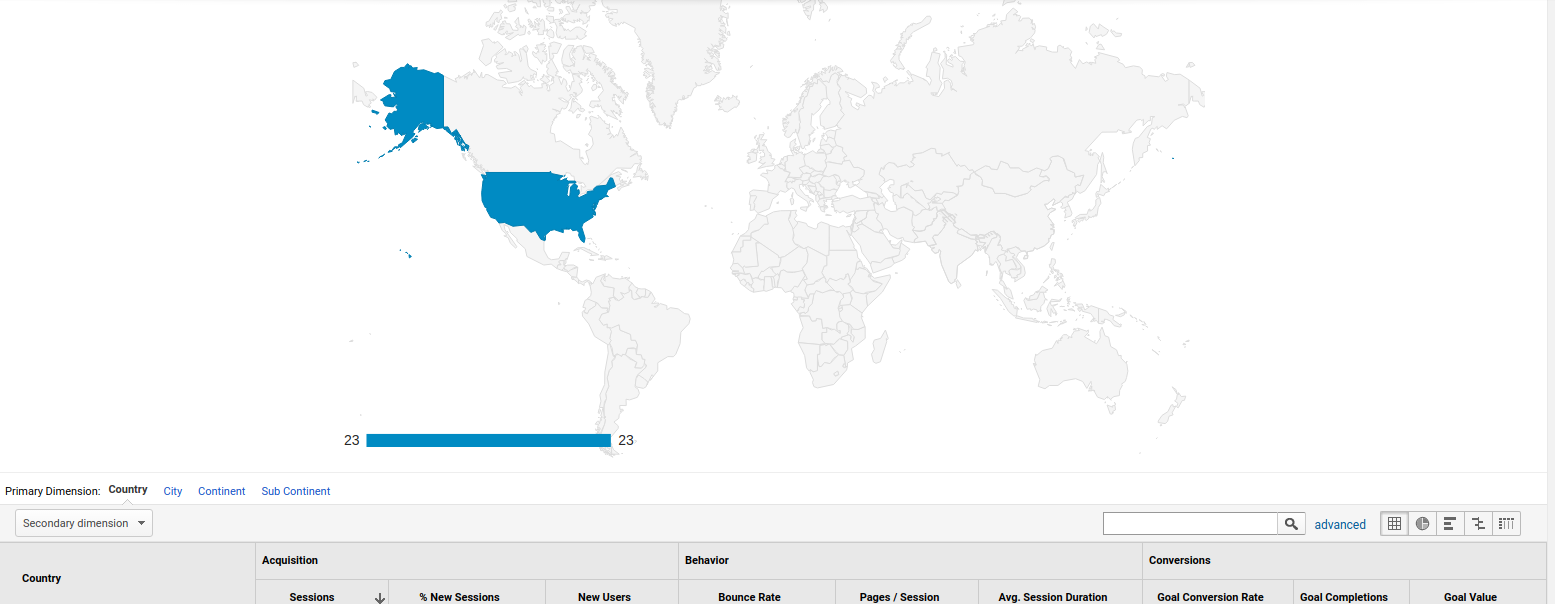
\includegraphics[scale = .5]{places.png}
\centering
\caption{Accessed by state }
\end{figure}
In \textbf{Figure 3}, we see that most of the users are from PA and CA. You may also toggle with the primary dimension, so if the user wants to go ahead and look at the city, all that would be have to be done is click on the city. 
\begin{figure}[t]
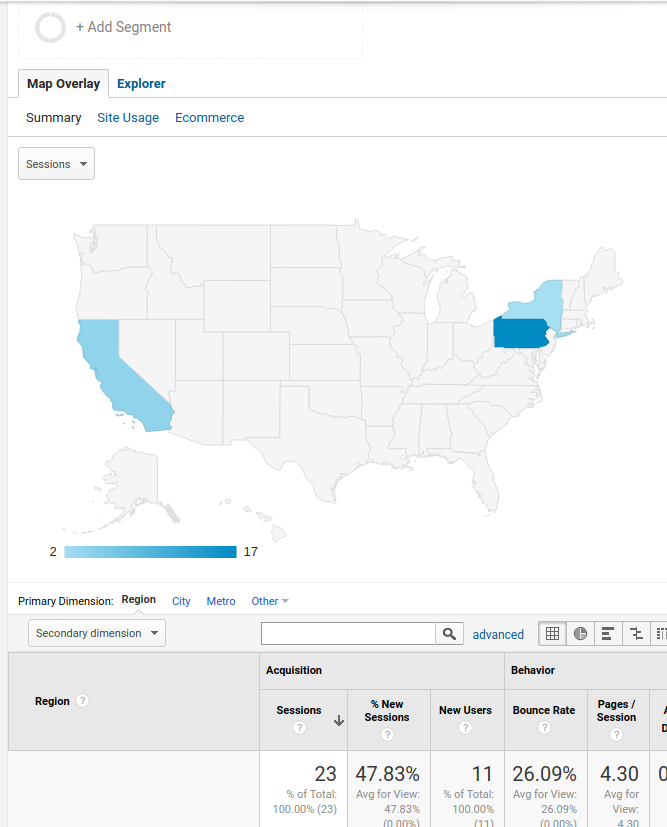
\includegraphics[scale = .5]{city.png}
\centering
\caption{Accessed by state }
\end{figure}
Now if we want to look at the user, in the form what they were interested in the website we would just look at the pages they looked and how many times. If you go down in location overview you can see that there is a section that says page, in that section we the different pages of the website. 
the most viewed page is obviously be the first one. In \textbf{Figure 4 } We have a page were we get to see what pages were viewed by all the users. 
 
\begin{figure}[t]
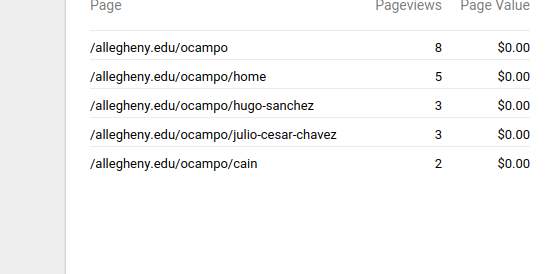
\includegraphics[scale = .5]{pages.png}
\centering
\caption{Pages viewed}
\end{figure}

Now if we want to see what our bounce rate is we can look at going back to \textbf{figure 3}, The problem you should note that if no one is looking at your site it can give you a 0 percent bounce rate, and there give would be no use. Now if you want the unique user all you would have to do is look at the client ID, The client ID is found in audience where the user explorer would then direct you to all of the users that have used your website. In \textbf{Figure}, 5  there were about 10 people who used my website. The problem that we should note is that there maybe a user that can have  multiple devices and therefore. 

\begin{figure}[t]
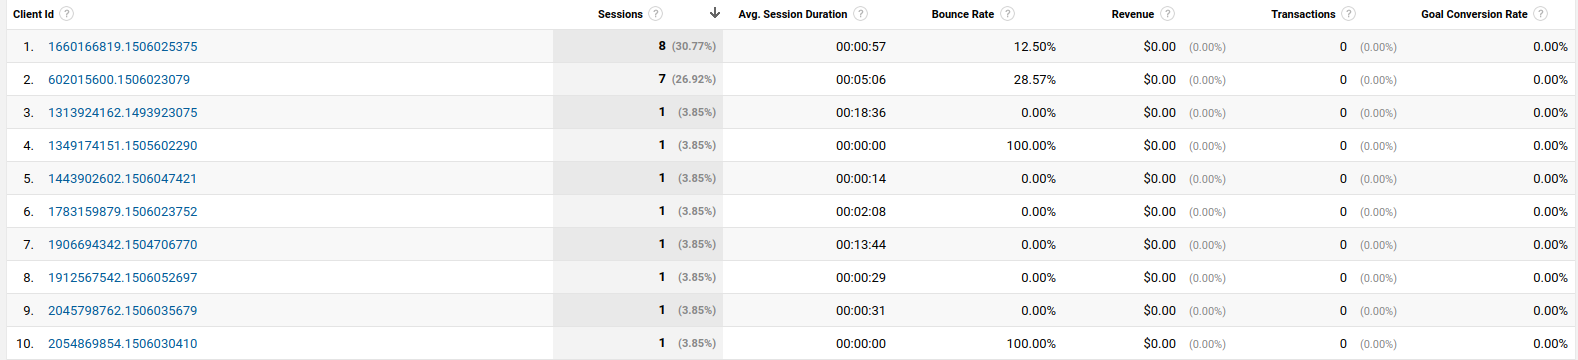
\includegraphics[scale = .5]{unique.png}
\centering
\caption{Unique views}
\end{figure}

In \textbf{Figure 5}, we can also see that the average duration of the users, so for the first user used the website for an average of about a minute. 

Now if we want to see what percentage of the users are new to those that are not, we would go to audience and then go to overview in the overview we will be able to see that 50 percent are new users and 50 percent are returning users.  while also calculating the total page views, sessions, avg session duration, bounce rate. 
   
\begin{figure}[t]
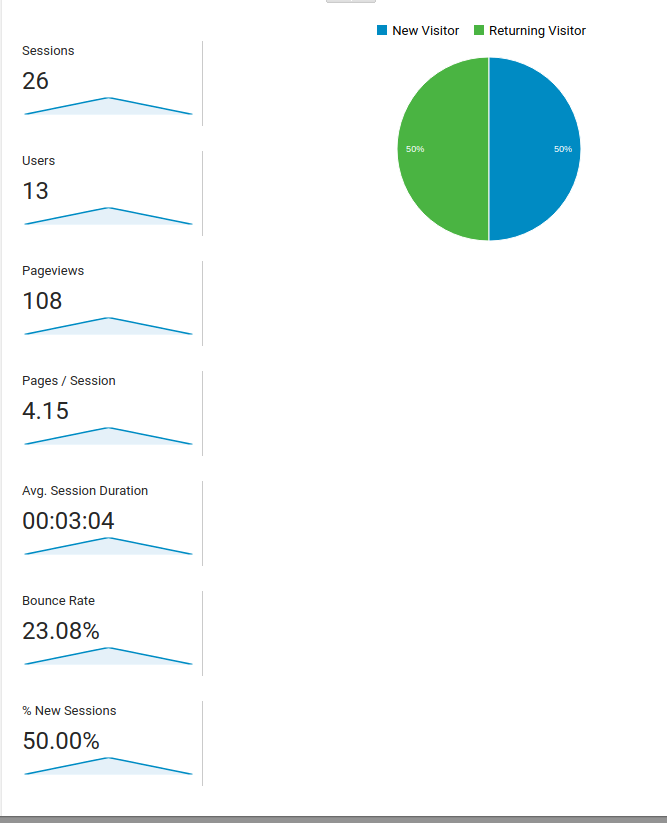
\includegraphics[scale = .5]{newuser.png}
\centering
\caption{views}
\end{figure}

Now if want to know where are traffic is coming from we can look go to all traffic and pick on source/medium and it will tell you where all of your users are coming from. For example, in \textbf{Figure 7}, we see that most of the users are coming from Facebook or coming directly.

\begin{figure}[t]
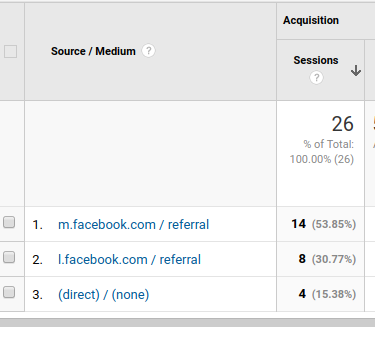
\includegraphics[scale = .5]{traffic.png}
\centering
\caption{Traffic}
\end{figure}

\newpage
\section{questions after tutorial}
\begin{itemize}
    \item For a web site such as www.amazon.com, which one metric is the most important to determine the business performed daily by the site? Why? 
    
    I think the most important one would be the bounce rate because if you want to sell things the business wants the user to stay longer and therefore have a higher chance of buying an item. 
    
\item For a web site such as www.facebook.com, which one metric is the most important for determining the general ease of use of the site. Why?
The demographics, maybe the age of the users, so if like 13 year can use it has been made pretty easy. 

\item What metric would you suggest is often included in a report but is, actually, not very informative or provides no real value to an analysis? Why?
I think the new users because a user may have multiple devices but we should also note that, if there is no users the bounce rate maybe 0 percent so this could be misleading in the sense that you think you are doing good, but in reality you have no users.  

\end{itemize}

\end{document}

